\documentclass{beamer}

\usepackage{color}
\definecolor{TUCgreen}{HTML}{779a2b}

\usetheme{Madrid}
\usecolortheme[named=TUCgreen]{structure}
%\usecolortheme{lily}	% Farbtheme

\setbeamertemplate{itemize items}[square]
\setbeamertemplate{enumerate items}[square]
\setbeamertemplate{section in toc}[square]
\setbeamerfont{section number projected}{size=\normalsize}


%\setbeamercolor{frametitle}{bg=TUCgreen}
%\setbeamercolor{headline}{bg=red}

\usepackage[utf8]{inputenc}
\usepackage[german]{babel}
\usepackage{amsmath}
\usepackage{amsfonts}
\usepackage{amssymb}
\usepackage{graphicx}
\author[Eric Kunze]{Eric Kunze}
%\title{
\includegraphics[height=2cm]{Rust_Logo.eps}\\Rust in the Web}
\title[]{Rust in the Web}
%\setbeamercovered{transparent} 
\setbeamertemplate{navigation symbols}{} 
%\logo{
\includegraphics[height=1cm]{Rust_Logo.eps}} 
%\institute{TU Chemnitz} 
\date{04.11.2015} 
\date{} 
%\subject{Zwischenvortrag} 

\usepackage{textpos}

\usepackage{listings}

\usepackage{listings}
\usepackage{color}

\definecolor{mygreen}{rgb}{0,0.6,0}
\definecolor{mygray}{rgb}{0.5,0.5,0.5}
\definecolor{mymauve}{rgb}{0.58,0,0.82}

\lstset{ %
  backgroundcolor=\color{lightgray!50},   % choose the background color; you must add \usepackage{color} or \usepackage{xcolor}
  basicstyle=\scriptsize,        % the size of the fonts that are used for the code
  breakatwhitespace=false,         % sets if automatic breaks should only happen at whitespace
  %breaklines=true,                 % sets automatic line breaking
  captionpos=b,                    % sets the caption-position to bottom
  commentstyle=\color{orange},    % comment style
  deletekeywords={...},            % if you want to delete keywords from the given language
  escapeinside={\%*}{*)},          % if you want to add LaTeX within your code
  extendedchars=true,              % lets you use non-ASCII characters; for 8-bits encodings only, does not work with UTF-8
  %frame=single,	                   % adds a frame around the code
  keepspaces=false,                 % keeps spaces in text, useful for keeping indentation of code (possibly needs columns=flexible)
  keywordstyle=\color{mygreen},       % keyword style
  language=c,                 % the language of the code
  otherkeywords={fn,mut,Vec,vec!,let,i32,in,println!},           % if you want to add more keywords to the set
  numbers=left,                    % where to put the line-numbers; possible values are (none, left, right)
  numbersep=3pt,                   % how far the line-numbers are from the code
  numberstyle=\tiny\color{mygray}, % the style that is used for the line-numbers
  rulecolor=\color{black},         % if not set, the frame-color may be changed on line-breaks within not-black text (e.g. comments (green here))
  showspaces=false,                % show spaces everywhere adding particular underscores; it overrides 'showstringspaces'
  showstringspaces=false,          % underline spaces within strings only
  showtabs=false,                  % show tabs within strings adding particular underscores
  stepnumber=1,                    % the step between two line-numbers. If it's 1, each line will be numbered
  %stringstyle=\color{mymauve},     % string literal style
  tabsize=2,	                   % sets default tabsize to 2 spaces
  title=\lstname                   % show the filename of files included with \lstinputlisting; also try caption instead of title
}


\usepackage{multirow}
\usepackage{setspace}



\begin{document}

\begin{frame}{\centerline{Proseminar Web Engineering}}
	\begin{center}
		
\includegraphics[height=3cm]{Rust_Logo.eps}\\~\\
		\Large \textbf{Rust in the Web}\\~\\
		\normalsize Eric Kunze
	\end{center}
 \end{frame}
 

\addtobeamertemplate{frametitle}{}{%
\begin{textblock*}{10cm}(.74\textwidth,-.95cm)
	\begin{minipage}[c]{0.24\textwidth}
		\footnotesize Rust in the Web 
	\end{minipage}
	\begin{minipage}[c]{0.2\textwidth}
		
\includegraphics[height=.8cm]{Rust_Logo.eps}
	\end{minipage}
\end{textblock*}}

\begin{frame}{Inhalt}

\tableofcontents

\end{frame}

%\begin{frame}{Title}
%	Inhalt
%	\begin{itemize}
%	  \item Test
%	  \item Test
%	\end{itemize}
%\begin{block}{Blocktitel}		% normaler Block
%	 Blockinhalt
%\end{block}
% 
%\begin{exampleblock}{Blocktitel}	% Beispielblock
%	 Blockinhalt
%\end{exampleblock}
% 
%\begin{alertblock}{Blocktitel}		% Warnblock
%	 Blockinhalt
%\end{alertblock}
%\end{frame}

\section{Entstehungsgeschichte}

\begin{frame}{Entstehungsgeschichte}
	\begin{itemize}
	  \item 2006 Projekt von Graydon Hoare
	  \item ab 2009 Projekt bei Mozilla
	  \item 15. Mai 2015 Veröffentlichung der Version 1.0
	  \pause
	  \item[]
	  \item Entwicklung einer neuen Browserenging $\rightarrow$ Servo
	  \pause
	  \begin{itemize}
		\item Warum nicht C\texttt{++} oder Java?
	  \end{itemize}
	 \end{itemize}	 
\end{frame}

%\section{Was unterscheidet Rust von anderen Programmiersprachen?}
\section{Ziele von Rust}
\begin{frame}{Ziele von Rust}
Rust: Safe System Programming
	  \begin{itemize}
	  	  \pause
	      \item Performance
	      \pause
	      \item Kontrolle 
	      \begin{itemize}
	          \item minimale Runtime
	          \item keine Garbage Collection
	      \end{itemize}
	      \pause
	      \item Sicherheit      
	      \pause
	      \item Parallelität
	      \pause
	      \item Features von höheren und funktionalen Programmiersprachen
	      \begin{itemize}
	        \item Pattern Matching
	        \item Traits
	        \item Closures
	      \end{itemize}
	  \end{itemize}
\end{frame}

\section{Ownership and Borrowing}

\begin{frame}[fragile]{Ownership and Borrowing}
	\begin{itemize}
	\pause
	    \item Ownership
	    \begin{itemize}
	        \item jede Ressource hat zu einem Zeitpunkt \textbf{genau einen} Besitzer
	        \item Ressourcen können den Besitzer wechseln
	        \pause
	    \end{itemize}    
	\end{itemize}
\begin{center}
\hspace{3pt}
\begin{minipage}[t]{.47\textwidth}
\begin{lstlisting}
fn foo() {	
  let mut y: Vec<i32> 
      = Vec::new();
		
  y.push(4);	
  bar(y);	
  y.push(5); // Compiler Error	
}
\end{lstlisting}				
\end{minipage}
%\hfill
\hspace{3pt}
\begin{minipage}[t]{.47\textwidth}
\begin{lstlisting}
fn bar(x: Vec<i32>) {	
  ...
}
\end{lstlisting}				
\end{minipage}
\end{center}
\end{frame}

\begin{frame}[fragile]{Ownership and Borrowing}
	\begin{itemize}
	    \item Borrowing
	    \begin{itemize}
	        \item Ownership kann verliehen werden
	    \end{itemize}
	    \item[]
	    \pause
	    \item shared borrow  
	    \begin{itemize}
	      \item der Besitzer dieser Referenz kann die Ressource \textbf{nicht verändern} 
	      %die Referenz ist \textbf{unveränderlich}
	      \item die Ressource kann \textbf{mehrfach} verliehen werden
	      \pause
	    \end{itemize}
	\end{itemize}
\begin{center}
\hspace{3pt}
\begin{minipage}[t]{.47\textwidth}
\begin{lstlisting}
fn foo() {	
  let mut y: Vec<i32> 
      = Vec::new();
		
  y.push(4);	
  bar(&y);	
  y.push(5); // Ok
}
\end{lstlisting}				
\end{minipage}
\hspace{3pt}
\begin{minipage}[t]{.47\textwidth}
\begin{lstlisting}
fn bar(x: &Vec<i32>){
  ...	
  b = a + x[0];  // Ok	
	
  x.push(1); // Compiler Error
	
}
\end{lstlisting}				
\end{minipage}
\end{center}
\end{frame}


\begin{frame}[fragile]{Ownership and Borrowing}
	\begin{itemize}
	    \item mutable borrow  
	    \begin{itemize}
	        \item zu einem Zeitpunkt darf \textbf{nur eine} Referenz existieren      
	        \item der Besitzer dieser Referenz kann die Ressource \textbf{verändern}
	        \pause
	    \end{itemize}
	\end{itemize}
\begin{center}
\hspace{3pt}
\begin{minipage}[t]{.48\textwidth}
\begin{lstlisting}
fn foo() {	
  let mut y 
      = vec![1,2,3,4,5];
  let mut x: Vec<i32> 
      = Vec::new();
		
  bar(&y, &mut x); // Ok
  bar(&y, &mut y); 
      // Compiler Error
}
\end{lstlisting}				
\end{minipage}
\hspace{3pt}
\begin{minipage}[t]{.47\textwidth}
\begin{lstlisting}
fn bar(y: &Vec<i32>, 
       x: &mut Vec<i32>){
	
  for v in y{
    x.push(*v);
  }
}
\end{lstlisting}				
\end{minipage}
\end{center}
\end{frame}

\section{Vor- und Nachteile von Rust}

\begin{frame}{Vor- und Nachteile von Rust}
\pause
\begin{minipage}[t]{.46\textwidth}
Vorteile
\begin{itemize}
  \item Sicherheit und Geschwindigkeit
  \item Tools
  \begin{itemize}
    \item Cargo
    \item rustdoc
  \end{itemize}
  \item Open Source Projekte \\ crates.io
\end{itemize}
\end{minipage}
\hfill
\begin{minipage}[t]{.46\textwidth}
\pause
Nachteile
\begin{itemize}
  \item sehr junge Sprache
  \item häufige Änderungen 
  \item Dokumentation   
  \item (Kompilierzeit)
\end{itemize}
\end{minipage}
\end{frame}

%\begin{frame}[fragile=singleslide]{Was macht Rust sicher?}
%\begin{itemize}
%    \item Aliasing und Mutation zur gleichen Zeit wird verhindert
%   	\item Bsp. C\texttt{++}   	
%\end{itemize}
%\begin{center}
%\hspace{3pt}
%\begin{minipage}[t]{.47\textwidth}
%\begin{lstlisting}[language=C++,otherkeywords={}]
%void foo(){ 
%	int *y = new int[10];	
%	for(int i=0;i<10;i++)
%		y[i] = i;
%
%	int *x = &y[9];
%	y=bar(y);	
%	delete[] y;		
%	cout<<*x<<endl;
%}
%\end{lstlisting}				
%\end{minipage}
%\hspace{3pt}
%\begin{minipage}[t]{.47\textwidth}
%\begin{lstlisting}[language=C++,otherkeywords={}]
%int* bar(int *v){
%	delete[] v;	
%	v = new int[5]	
%	for(int i=0;i<10;i++){
%		v[i] = i*2;
%	}	
%	return v;
%}
%\end{lstlisting}				
%\end{minipage}
%\end{center}
%\end{frame}

\section{Rust in the Web}

\begin{frame}{Rust in the Web}

\begin{minipage}[t]{.45\textwidth}
\begin{itemize}
  \item HTTP-Server
  \begin{itemize}
    \item Hyper
    \item tiny-http
  \end{itemize}
  \item []
  \item HTTP client
  \begin{itemize}
    \item Hyper
    \item curl-rust
  \end{itemize} 
  \item []
  \item Database drivers
  \begin{itemize}
    \item rust-postgres
    \item rusqlite
    \item redis-rs
  \end{itemize}
\end{itemize}
\end{minipage}
\hfill
\begin{minipage}[t]{.45\textwidth}
\begin{itemize}
\item Frameworks
  \begin{itemize}
    \item Iron
    \item rustful
    \item Nickel
  \end{itemize}  
\end{itemize}
\end{minipage}

\end{frame}

\section{Iron}
\begin{frame}{Iron}
\begin{itemize}
    \item Server Framework
    \item basiert auf Hyper
    \item Multithreaded
    \item Basisframework ist leicht erweiterbar
    \item bietet eine Infrastruktur, um das Framework an individuelle Bedürfnisse anzupassen
\end{itemize}
\end{frame}





\section{Demo}
\begin{frame}[fragile]{Demo}
\begin{center}
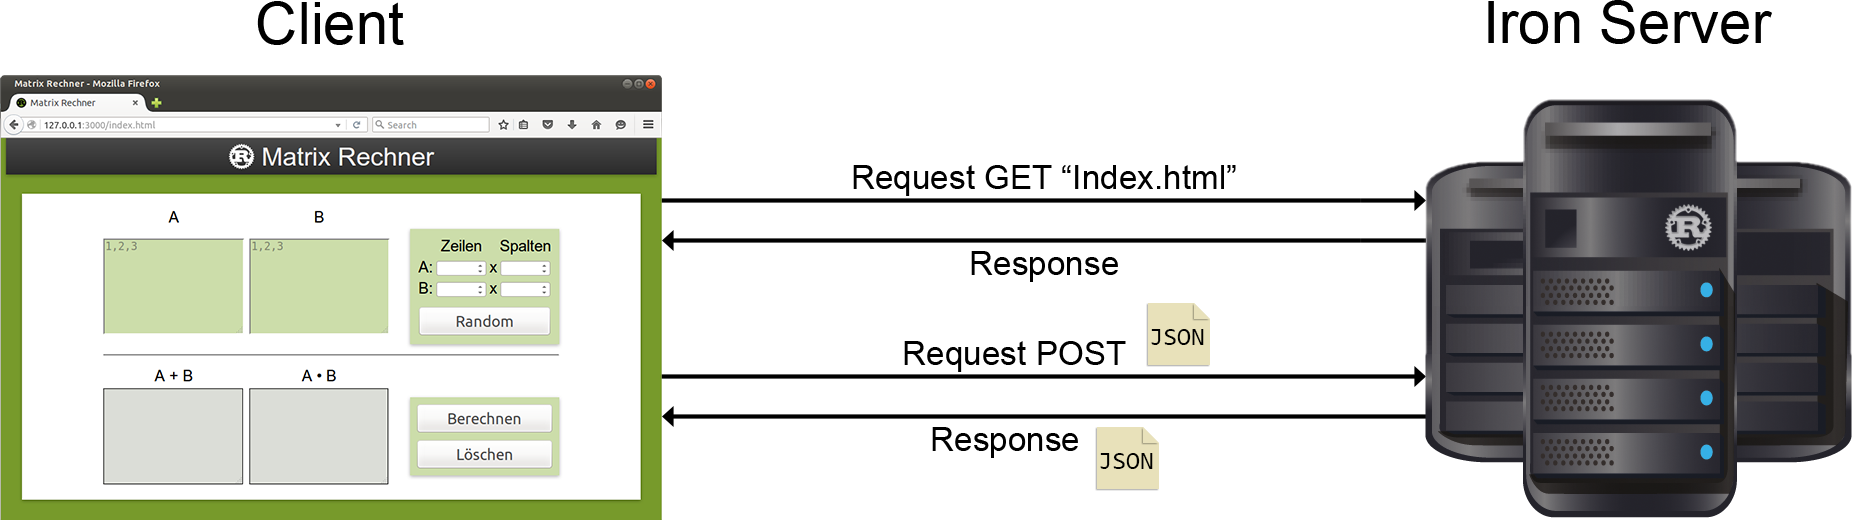
\includegraphics[width=0.8\textwidth]{uebersicht.png}
\vspace{1cm}
\pause
\begin{minipage}[t]{.4\textwidth}
{\scriptsize Request Body}
\begin{lstlisting}
{
 "mat_a":{
   "rows": 3,
   "cols": 3,
   "elem": ["1","2",...]},
 "mat_b":{...}
}
\end{lstlisting}				
\end{minipage}
\hspace{2cm}
\begin{minipage}[t]{.3\textwidth}
{\scriptsize Response Body}
\begin{lstlisting}
{
 "message":"Fehler",
 "mat_a":{...},
 "mat_b":{...}
}
\end{lstlisting}				
\end{minipage}

\end{center}
\end{frame}
\begin{frame}{Demo}
\begin{center}
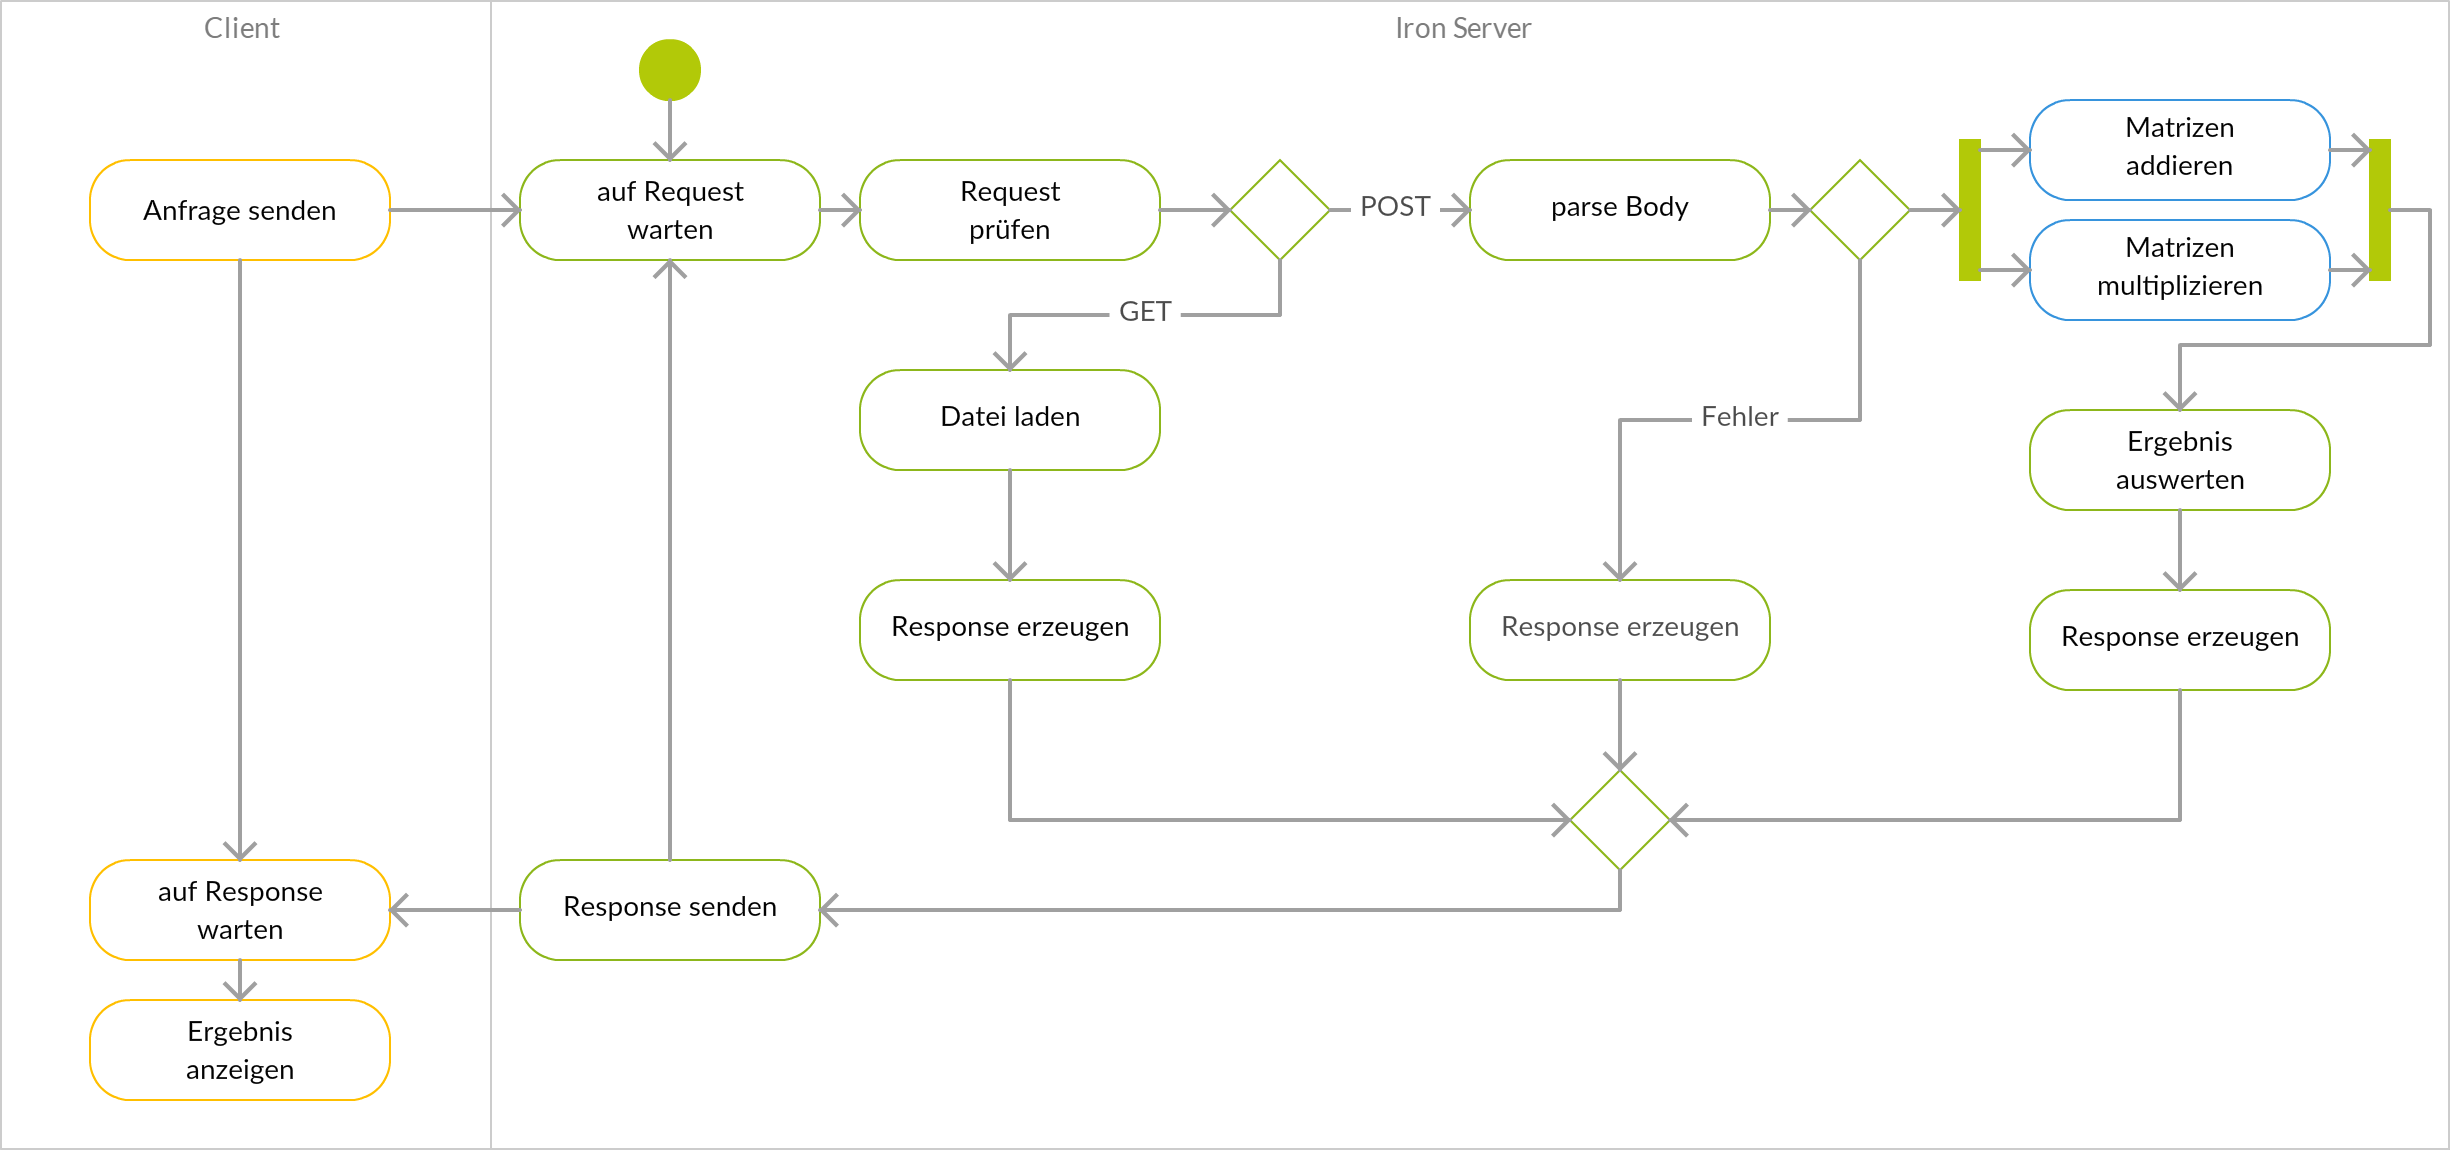
\includegraphics[width=\textwidth]{Iron_Server.png}
\end{center}
\end{frame}

\begin{frame}{Quellen}
	\begin{itemize}
	  \item doc.rust-lang.org
	  \item rustbyexample.com
	  \item[]
	  \item arewewebyet.com
	  \item ironframework.io
	  \item[]
	  \item[] 
\includegraphics[height=3.5mm]{youtube_logo.eps}
	  	\begin{itemize}
	  	\item GoogleTechTalks - The Rust Programming Language \\ (Alex Crichton, 06.06.2015)
	  	\item stanfordonline - The Rust Programming Language  \\ (Aaron Turon, 12.03.2015)
	  	\item Linux.conf.au 2015 - Servo: Building a Parallel Browser \\ (Jack Mofitt, 16.01.2015)
	  	\end{itemize}
	\end{itemize}
\end{frame}
\end{document}